\documentclass[conference]{IEEEtran}

\ifCLASSINFOpdf
   \usepackage[pdftex]{graphicx}
  % declare the path(s) where your graphic files are
  % \graphicspath{{../pdf/}{../jpeg/}}
  % and their extensions so you won't have to specify these with
  % every instance of \includegraphics
   \DeclareGraphicsExtensions{.pdf,.jpeg,.png}
\else
  % or other class option (dvipsone, dvipdf, if not using dvips). graphicx
  % will default to the driver specified in the system graphics.cfg if no
  % driver is specified.
   \usepackage[dvips]{graphicx}
  % declare the path(s) where your graphic files are
  % \graphicspath{{../eps/}}
  % and their extensions so you won't have to specify these with
  % every instance of \includegraphics
   \DeclareGraphicsExtensions{.eps, .ps}
\fi

\hyphenation{}


\begin{document}

\title{Data Layout for Distributed Numerical Python}

% author names and affiliations
% use a multiple column layout for up to three different
% affiliations
\author{\IEEEauthorblockN{Mads Ruben Burgdorff Kristensen}
\IEEEauthorblockA{eScience Centre\\
University of Copenhagen\\
Denmark}
\and
\IEEEauthorblockN{Brian Vinter}
\IEEEauthorblockA{eScience Centre\\
University of Copenhagen\\
Denmark}}

% make the title area
\maketitle

\begin{abstract}

\end{abstract}

\IEEEpeerreviewmaketitle

\section{Introduction}
In this paper we introduce generic latency hiding for Distributed Numerical Python (DistNumPy)\cite{distnumpy09}, which is a library for doing numerical computation in Python that targets scalable distributed memory architectures. DistNumPy extends the NumPy module\cite{numpy}, which is popular for scientific programming. Replacing NumPy with DistNumPy enables the user to write sequential Python programs that seamlessly utilize distributed memory architectures.

Communication latency hiding is well known technique to improve the performance and scalability of communication bound problems. We define latency hiding informally as in \cite{Strumpen94latencyhiding} -- ``a technique to increase processor utilization by transferring data via the network while continuing with the computation at the same time''

There exist a lot of methods to implement latency hiding and most of them are tailored to a particular problem. The current method used in DistNumPy to hide the communication latency is also tailored to a particular problem -- namely an element-by-element computation on distributed arrays that uses identical distribution schemes. However, a broad range of DistNumPy programs make use of distributed arrays that do not share identical distribution schemes. In this paper we therefore introduce a generic method for latency hiding that is not tailored to any particular problem.


\subsection{Motivation}


\section{Data Layout}
The data layout used in DistNumPy consists of three levels (Fig. \ref{fig:view_block}). The first level is the base-block level, in which a base-block map directly into one block of memory located on one node. The memory block is not necessarily contiguous but only one MPI-process has exclusive access to the block. A base-block is the basic build block in the distribution scheme used when distributing DistNumPy arrays across multiple MPI-processes.

The second level is the view-block level, which is an abstraction level above the base-block level. A view-block represents a basic block of an array-view, which means that a view-block is a contiguous block of array elements from the perspective of the user. A view-block can span over multiple base-blocks and consequently also over multiple MPI-processes. For a MPI-process to access a whole view-block it will have to fetch data from possible remote MPI-processes and put the pieces together before accessing the block. To avoid this process, which may require some internal memory copying, we divide view-blocks into sub-view-block.

Sub-view-block is the third block level and is simply a block of data that is a part of a view-block but is located in only one MPI-process. The general idea is that all array operation is translated into a number of sub-view-block operations.

\begin{figure}
 \centering
 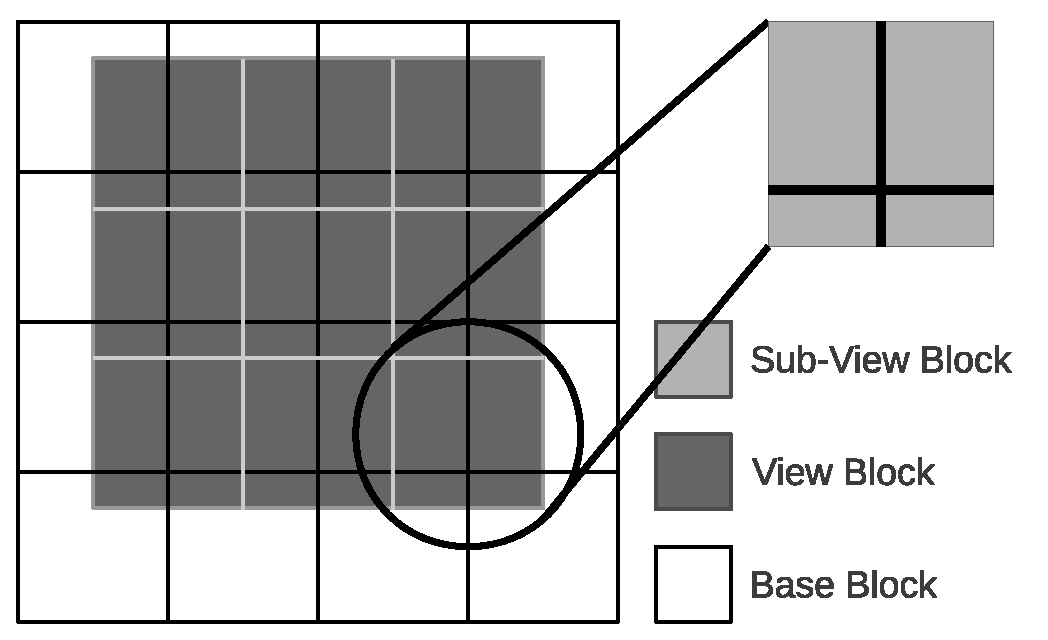
\includegraphics[width=150px]{gfx/view_blocks}
 \caption{An illustration of the block hierarchy used in representing a 2D distributed array. The array is divided into three block-types: Base, View and Sub-View blocks. The 16 base-blocks make up the base-array, which may be distributed between multiple MPI-processes. The 9 view-blocks make up a view of the base-array and represent the elements that are visible to the user. Each view-block is furthermore divided into four sub-view-blocks, which are the basic block of elements and is always located on one MPI-process.}
 \label{fig:view_block}
\end{figure}


\subsection{Base-block Distribution}
\begin{figure}
 \centering
 \includegraphics[width=\linewidth]{gfx/datalayout}
 \caption{The Two-Dimensional Block Cyclic Distribution of a matrix on a 2 x 3 grid of processors.}
 \label{fig:datalayout}
\end{figure}

Two-Dimensional Block Cyclic Distribution is a very popular distribution scheme and it is used in numerical libraries like ScaLAPACK\cite{Blackford96} and LINPACK\cite{linpack79}. It supports matrices and vectors and has a good load balance in numerical problems that have a diagonal computation workflow e.g. Gaussian elimination. The distribution scheme works by arranging all MPI-processes in a two dimensional grid and then distributing data-blocks in a round-robin fashion either along one or both grid dimensions (Fig. \ref {fig:datalayout}); the result is a well-balanced distribution.

NumPy is not limited to matrices and vectors as it supports arrays with an arbitrary number of dimensions. DistNumPy therefore use a more generalized N-Dimensional Block Cyclic Distribution inspired by High Performance Fortran\cite{Loveman93}, which supports an arbitrary number of dimensions. Instead of using a fixed process grid, we have a process grid for every number of dimensions. This works well when operating on arrays with the same number of dimensions but causes problems otherwise. For instance in a matrix-vector multiplication the two arrays are distributed on different process grid and may therefore require more communication. ScaLAPACK solves the problem by distributing vectors on two-dimensional process grids instead of one-dimensional process grids, but this will result in vector operations that cannot utilize all available processors. An alternative solution is to redistribute the data between a series of identically leveled BLAS operations using a fast runtime redistribution algorithm like \cite{PrylliT97} demonstrates.




\section{Lazy Evaluation}




Lazy evaluation on these data blocks are managed through a simple dependency list for each block. When a NumPy operation is issued it is split across the sub-view blocks that are involved in the operation. For each such operation on a sub-view block a set of tasks are created, one for each combined set of data-blocks to sub-view blocks. Dependencies are then added to the dependency-list of each data-block that is involved, each dependency link back to the individual tasks. When the number of dependencies on a task reached zero the task may be moved to the ready-queue. But before this is done we traverse the dependency list and include any other task that can be merged into the ready task, given that they could execute in parallel with the task or could execute given the task was done, when two tasks are merged into one, the remaining list is traversed under the same rules but for the merged task.


\subsection{Apply Operation List}




\section{Examples}


\section{Experiments}


\section{Future work}


\section{Conclusions}


\bibliographystyle{IEEEtran}
\bibliography{/home/madsbk/repos/priv/diku/phd/paper_archive/main}

\end{document}